\section{Grundlagen}

\subsection{Überblick}
Um unseren Lösungsansatz nachvollziehen zu können, ist es erforderlich, 
die Problemstellung detailliert zu analysieren. Im ersten Schritt wird betrachtet, 
welche Zielgruppe Ludwig System anspricht und welche spezifischen Optimierungen 
das Unternehmen verfolgt. Im Anschluss werden bestehende Lösungsansätze verglichen, 
um deren Stärken und Schwächen zu bewerten und als Grundlage 
für die Entwicklung eines verbesserten Systems zu nutzen.



\subsubsection{Anwendungsdomäne}
Das Abhängen von Lasten per Hand ist nicht nur zeitaufwendig, sondern oft auch gefährlich. 
Ludwig System bietet mit ihren funkgesteuerten Lasthaken eine innovative Lösung, 
die diese Arbeit deutlich erleichtert. Diese Haken ermöglichen es den Mitarbeitenden, 
Lasten aus sicherer Entfernung anzuheben und auszubalancieren. Besonders beliebt ist 
die Traverse, die speziell für den Transport von Dachelementen und Wänden entwickelt wurde. 
Allerdings müssen aktuelle Versionen noch manuell an die Last befestigt werden, 
was besonders bei hohen Wänden zeitaufwendig und gefährlich sein kann. 
Abbildung 2.2 illustriert die Nutzung der Traverse beim Transport eines Dachelements.


\begin{figure}[H]
    \centering
    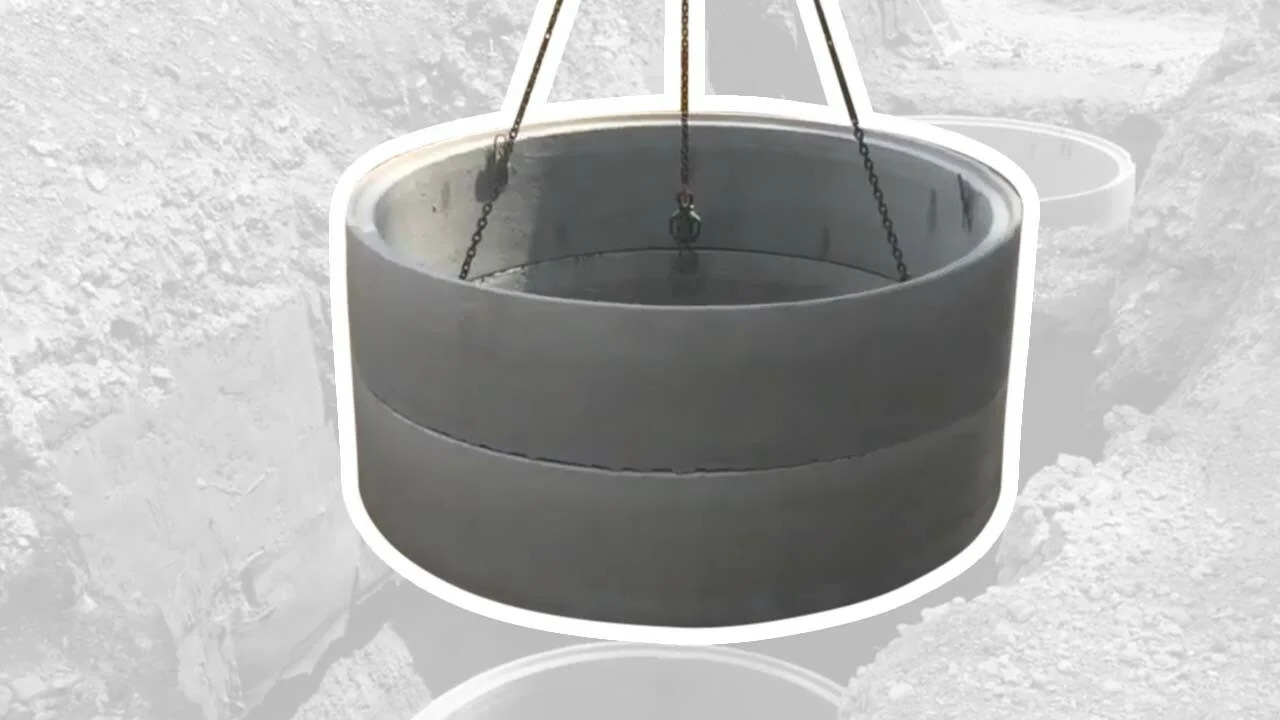
\includegraphics[width=0.5\textwidth]{graphics/Betonelement.jpg}\hfill%
    \caption{Ludwig Hook mit Betonelement}
    \centering
    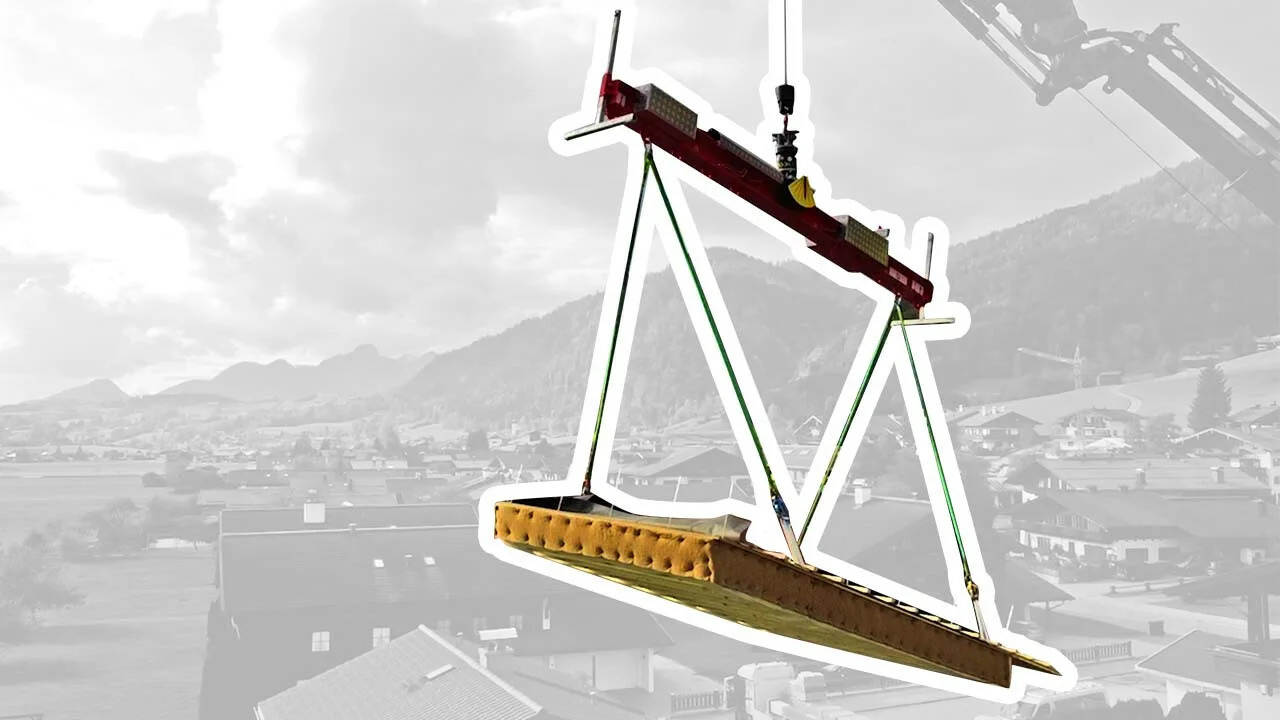
\includegraphics[width=0.5\textwidth]{graphics/Traverse.jpg}
    \caption{Traverse mit Dachelement}
\end{figure}

\subsubsection{Last}
Unter Lasten sind vor allem Fertigstrukturen wie z.B. Fertig erstellte Wände oder Dächer. Lasten haben maximal 2 Anschlagspunkte, welche einen Abstand von 1m bis 6m zueinander haben. Diese Anschlagspunkte können auf unterschiedliche Höchen sein, wie z.B. bei Dächer welche eine Neigung besitzen.


\clearpage
\subsubsection{Traverse}
Die LudwigTraverse ist eine Spezialtraverse, die speziell für den Lastausgleich entwickelt 
wurde. Sie erweist sich insbesondere dann als nützlich, wenn die Anschlagpunkte 
falsch positioniert sind und dadurch der Schwerpunkt der Last nicht korrekt berücksichtigt wird. 
Dies kann zu einer schrägen Ausrichtung beim Anheben der Last führen \cite{ludwigTraverse}.

\begin{figure}[H]
    \centering
    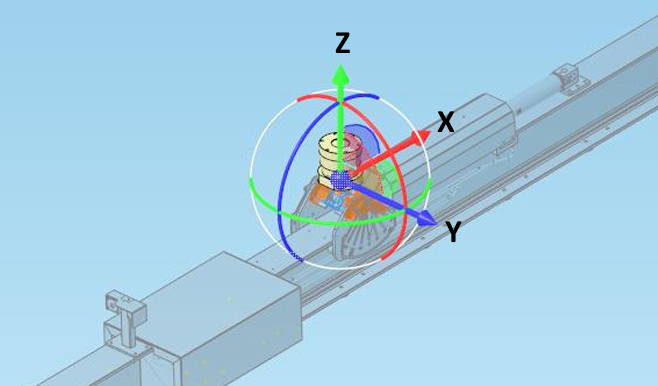
\includegraphics[width=0.5\linewidth]{graphics/Traverse_Rotationen.PNG}
    \caption{Koordinaten-System der Ludwig System Traverse}
    \label{fig:traverse}
\end{figure}

Abbildung \ref{fig:traverse} zeigt das linkshändige Koordinaten-System der Traverse.
Die Traverse hat Dimensionen (Länge × Breite y Höhe z) von 500 cm × 70 cm × 50 cm.
Dabei wird fortan die Rotation um die Y-Achse der Traverse als Neigen definiert und die Rotation 
um die Z-Achse der Traverse, als Rotieren definiert.


\subsection{Stand der Forschung}

\subsubsection{Arbeit: Objekterkennung und Distanzmessung für KollisionsVermeidung bei Lastenhebung}
(Arbeit: Object Detection and Distance Measurement Algorithm for Collision Avoidance of Precast Concrete Installation during Crane Lifting Process\cite{yong_object_2023} Erklären)

\subsubsection{Arbeit: Objekterkennung und 3D-basierte Objektortung für automatische Lastenhebung}
(Arbeit: Image-based onsite object recognition for automatic crane lifting tasks\cite{zhou_image-based_2021} Erklären)

\subsubsection{Arbeit: Erkennung von auf Robotersystemen angebrachten Passermarken}


\subsection{Passermarker}
\subsubsection{Einführung Passermarker}
\subsubsection{Posenschätzung durch AR Marker}
\subsubsection{Probleme mit Passermarkern}


\subsection{Objekterkennung durch Machine Learning}
\subsubsection{Grundlagen Objekterkennung mit Neuronalen Netzen}
\subsubsection{Vorhandene Modelle}
\subsubsection{Probleme mit Machine Learning}


\subsection{Kameras}
\subsubsection{Kameraeigenschaften}
(Erklären was FOV, Verzerrrungen etc ist)
\subsubsection{Intrinsische Kalibrierung}
\subsubsection{Herausforderungen}

\subsection{Vorhandene Frameworks}
(Erklärung von OpenCV und ihren Methoden)

